\documentclass[border=10pt]{standalone}
\usepackage{verbatim}
\usepackage{amsmath, calc}

\usepackage{tikz}
\usetikzlibrary{shapes, shadows, arrows}
\usetikzlibrary{positioning}
\usepackage{xcolor}

\begin{document}
    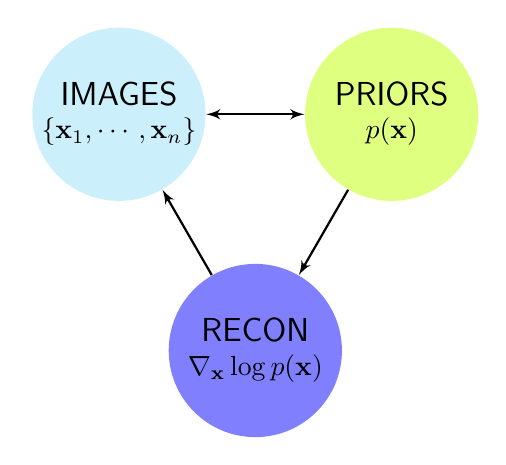
\begin{tikzpicture}\sffamily


        \begin{scope}[blend group = soft light]
            \node[fill=lime!50!white, circle, minimum size=2.2cm] (A) at  (30:2) {};
            \node[fill=cyan!20!white, circle, minimum size=2.2cm] (B) at  (150:2) {};
            \node[fill=blue!50!white, circle, minimum size=2.2cm] (C) at  (270:2) {};
        \end{scope}
        
        \node[inner sep=5pt, align=center]  at (30:2) {\large PRIORS \\ $p(\mathbf{x})$};
        \node[inner sep=5pt, align=center]  at (150:2) {\large IMAGES \\ $\{\mathbf{x}_1,\cdots,\mathbf{x}_n\}$};
        \node[inner sep=5pt, align=center]  at (270:2) {\large RECON \\ $\nabla_\mathbf{x}\operatorname{log}p(\mathbf{x})$};

        \draw[latex'-latex', thick, black] (A) to (B);
        \draw[-latex', thick, black] (A) to (C);
        \draw[-latex', thick, black] (C) to (B);
        
    \end{tikzpicture}
    
\end{document}